\documentclass[a4paper, 10pt]{jarticle}

\usepackage{amsmath}
\usepackage[dvipdfm]{graphicx}
\graphicspath{ {images/} }
\usepackage{subcaption}
\usepackage{stfloats}
\usepackage{enumerate}
\usepackage{latexsym}
\usepackage{times}
\usepackage[multi, deluxe]{otf}
\usepackage[title]{appendix}
\usepackage{subfiles}

\topmargin 0mm
\oddsidemargin -0.4mm
\evensidemargin -0.4mm
\textwidth 160mm
\textheight 237mm
\columnsep 7mm
\headheight 0mm
\footskip 10mm
\headsep 0mm
\partopsep 0mm
\textfloatsep 3mm
\intextsep 3mm

\title{
  \begin{flushright}
    \normalsize{
      九州大学 CPC Lab 研究会  \\
      2021年度 第13回 研究会資料 TR2021-013
    }
  \end{flushright}
  \Large{\textbf{\\プロセッサ設計演習}}
}
\author{
    ウン クアン イー\\
    九州大学 工学部 電気情報工学科 4年
}
\date{2021年07月05日}

\begin{document}
  \begin{twocolumn}

  \maketitle

  \section{はじめに} \label{section:introduction}
  \subfile{sections/introduction.tex}

  \section{プロセッサの仕様} \label{section:specifications}
  \subfile{sections/specifications.tex}

  \section{プロセッサの機能検証} \label{section:testing}
  \subfile{sections/testing.tex}

  \section{プロセッサの性能評価と論理合成} \label{section:evaluation}
  \subfile{sections/evaluation.tex}

  \section{プロセッサの性能改善方法と評価} \label{section:improvements}
  \subfile{sections/improvements.tex}

  \section{まとめ} \label{section:summary}
  \subfile{sections/summary.tex}

  \section*{謝辞}
  \subfile{sections/acknowledgement.tex}

  % won't be printed if nothing is cite
  \bibliography{reference.bib}
  \bibliographystyle{jplain}

  \onecolumn
  \clearpage
  \begin{appendices} \label{section:appendix}
    \section{プロセッサのブロック図} \label{section:block-diagram}
    \begin{figure}[h!]
      \centering
      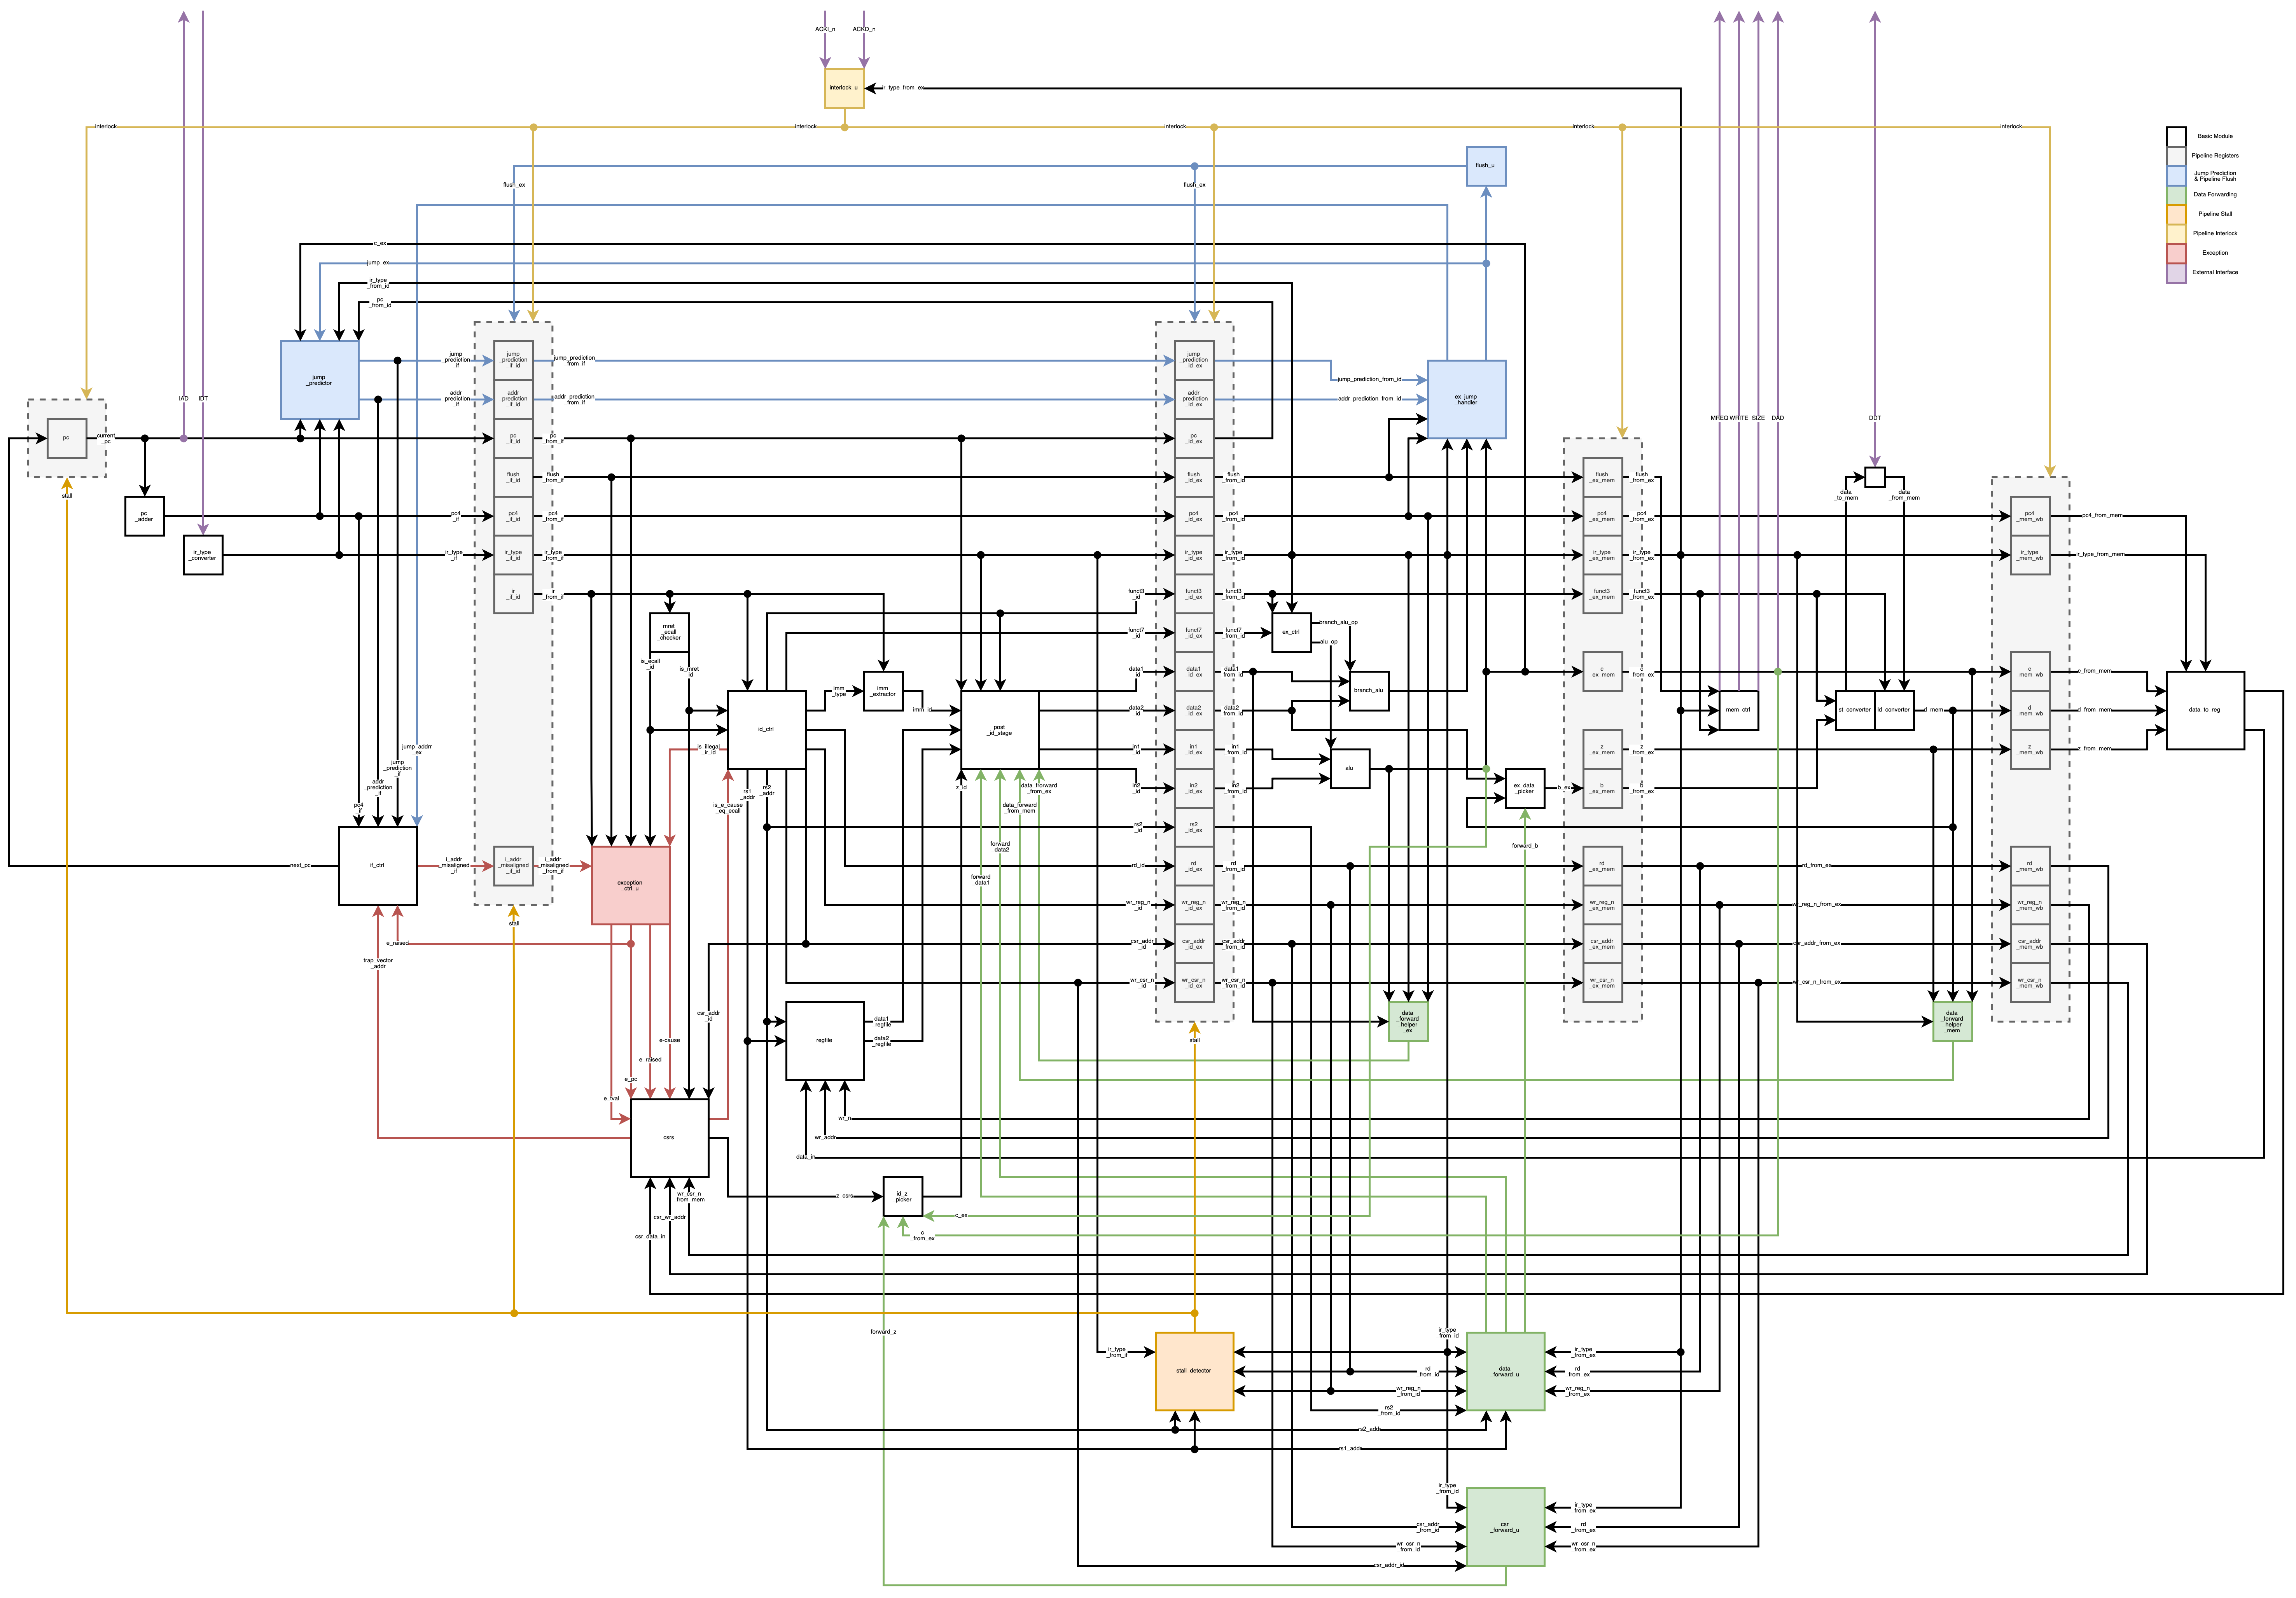
\includegraphics[angle=90, origin=c, totalheight=0.9\textheight]{images/block_diagram.png}
      \caption{プロセッサのブロック図}
      \label{fig:block-diagram}
    \end{figure}
  \end{appendices}

\end{twocolumn}
\end{document}
